\def\year{2022}\relax
%File: formatting-instructions-latex-2022.tex
%release 2022.1
\documentclass[letterpaper]{article} % DO NOT CHANGE THIS
\usepackage{aaai22}  % DO NOT CHANGE THIS
\usepackage{subcaption,times}  % DO NOT CHANGE THIS
\usepackage{helvet,color}  % DO NOT CHANGE THIS
\usepackage{courier}  % DO NOT CHANGE THIS
\usepackage[hyphens]{url}  % DO NOT CHANGE THIS
\usepackage{graphicx} % DO NOT CHANGE THIS
\urlstyle{rm} % DO NOT CHANGE THIS
\def\UrlFont{\rm}  % DO NOT CHANGE THIS
\usepackage{natbib}  % DO NOT CHANGE THIS AND DO NOT ADD ANY OPTIONS TO IT
\usepackage{caption} % DO NOT CHANGE THIS AND DO NOT ADD ANY OPTIONS TO IT
\DeclareCaptionStyle{ruled}{labelfont=normalfont,labelsep=colon,strut=off} % DO NOT CHANGE THIS
\frenchspacing  % DO NOT CHANGE THIS
\setlength{\pdfpagewidth}{8.5in}  % DO NOT CHANGE THIS
\setlength{\pdfpageheight}{11in}  % DO NOT CHANGE THIS
%
% These are recommended to typeset algorithms but not required. See the subsubsection on algorithms. Remove them if you don't have algorithms in your paper.
\usepackage{algorithm}
\usepackage{algorithmic}

%
% These are are recommended to typeset listings but not required. See the subsubsection on listing. Remove this block if you don't have listings in your paper.
\usepackage{newfloat}
\usepackage{listings,booktabs}
\lstset{%
	basicstyle={\footnotesize\ttfamily},% footnotesize acceptable for monospace
	numbers=left,numberstyle=\footnotesize,xleftmargin=2em,% show line numbers, remove this entire line if you don't want the numbers.
	aboveskip=0pt,belowskip=0pt,%
	showstringspaces=false,tabsize=2,breaklines=true}
\floatstyle{ruled}
\newfloat{listing}{tb}{lst}{}
\floatname{listing}{Listing}
%
%\nocopyright

 \begin{document}


\newcount\Comments  % 0 suppresses notes to selves in text
\Comments=0
\newcommand{\kibitz}[2]{\ifnum\Comments=1{\color{#1}{#2}}\fi}
\newcommand{\lel}[1]{\kibitz{blue}{[LEL:#1]}}
\newcommand{\kg}[1]{\kibitz{red}{[KG:#1]}}
\newcommand{\uf}[1]{\kibitz{green}{[UF:#1]}}



% The file aaai.sty is the style file for AAAI Press
% proceedings, working notes, and technical reports.
%
\title{Learning to Cooperate with People by Training with Interpretable Agents}
\author{Paper ID \#2956
}
\maketitle

\begin{abstract}
Reinforcement learning agents learn   strategies that optimize their utility in self-play settings,
but are known to be sub-optimal when interacting with agents using unknown strategies. This makes it challenging to design RL agents for interacting with partners without knowing whether they are people or other artificial agents that optimize for self play.
%This paper studies the design of reinforcement learning agents that interact with people in two-player cooperative games.
%Reinforcement learning (RL) agents traditionally optimize their strategy in self-play, but   agents using such strategies  are known to be suboptimal when cooperating  with people.
We propose to address this challenge by exposing  RL agent during training to  agents playing
 strategies that are interpretable to people.
We evaluate this approach in the  card game of Hanabi which is a popular domain for evaluating RL agents in cooperative settings.
We modified the training regime of
an  RL agent to include other  agents using   interpretable  strategies from the literature, which are hand-designed and rule-based.
%whose strategies are rule-based, deterministic, and succinct.
We hypothesized that exposing  RL agents to such strategies during training would improve their ability to cooperate with people, at a minimal cost to their self-play performance.
%\kg{Why? need to say stg about interpretable strategies here.}
We conducted a behavioral study in which we compared an RL agent
that was trained using our approach to a baseline  RL agent for playing Hanabi. We
show that that the augmented RL agent was able to significantly outperform the baseline RL agent when playing with people,
%higher than their performance when playing  with the  RL agent,
while only slightly reducing its performance in self play compared to the baseline TL agent. In a survey, participants reported they enjoyed playing the augmented agent more than the baseline RL agent, and that the augmented agent was easier to cooperate with.
%\kg{removed contribution statement, don't think it's warranted.}
%The contribution of this work is in showing how to augment existing RL agents to be human-compatible in cooperative sett without   having to redesign the agents from scratch.

% This work studies human-AI cooperation in two-player cooperative games. It was shown that this kind of cooperation is difficult and although the AI might achieve excellent results in self-play those don't always hold when attempting to cooperate with a human.
% Current approaches that tackle this issue include creating a mental model for the user and attempting to have the AI agent mimic it, trying to minimize the distance between its strategy and it, or provide post-hoc explanations about the reasons actions were taken.
% Creating an accurate mental model is difficult, and the performance of the resulting agent is limited by it. Additionally, it is not clear how to form and present explanations, and the number of them that people require to cooperate well with an agent might be very high.
% In this work, we try to tackle the problem by exposing reinforcement learning (RL) agents to understandable, rule-based strategies during training in order to make the resulting strategy easier for people to perform well with.
% We evaluate the approach in the card game of Hanabi and with a user study.
% The study measured how well humans performed with a regular RL agent compared to an RL agent trained according to the suggested changes. We found that humans were able to perform significantly better with the modified agent than with the regularly trained agent, while only slightly reducing the agent's performance in self-play.

\end{abstract}


\section{Introduction}

  Autonomous agents are increasingly deployed  in critical real world domains such as  autonomous vehicles and healthcare~\cite{navarro2017machine,wiens}.
  In such settings   participants' strategies are highly complex, yet they are required to cooperate with only partial or no knowledge of each other's strategy.  For example, a nurse  needs to provides the right tool at the right time  to a surgeon in an operating room, without receiving  explanations about how they are used at each point in the operation.
   Machine learning agents are commonly optimized for performance when interacting in self play (all agents use the same strategy) without directly reasoning about  people.
   This adversely affects their ability to collaborate with agents using unknown strategies---and people in particular.
   %This assumption may not hold in the real world where there is uncertainty about others' strategies.
   %However,
  %   Although an intelligent system might achieve excellent performance  when it is interacting in self play (when all agents share the same strategy), those don't always hold when attempting to interact
  % with   people~\cite{chattopadhyay2017evaluating}.
   %, whose strategies may differ widely from
%   those agents  used during training.
   A common example is the domain of  autonomous vehicles~\cite{nunes2018people}. It is much easier to program a vehicle that drives well on a road occupied solely by other vehicles that use the same driving conventions than having it adapt to human drivers~\cite{dresner2007sharing}.
 %To mitigate this problem  cooperation by explaining the AI's strategy to the human, but this is challenging to do for the class of ML models that are not symbolic, like Neural Networks~\cite{andrews1995survey}.

%Many settings require people and AI agents to cooperate. For example, autonomous robots are sometimes used to assist rescue works searching for survivors after an earthquake~\cite{ventura2012search,ito2016semi}.
%The robots themselves are not sufficient for the task, and cooperation with humans is essential for success. Effectively cooperating in this case is not easy. Humans and robots might search the same area if they are unaware of each other's search strategies. The human and robot should adapt their search strategies based on those of their partners to maximise efficiency.


% There exists a large body of work in the field of explainable AI~\cite{xu2019explainable}. Current approaches which tackle this issue include creating some kind of mental model for the user and attempting to have the AI agent mimic it~\cite{perez2015fast}, or try to minimize the distance between its strategy and it~\cite{kulkarni2019explicable}. Another kind of approach was to have the AI agent provide post-hoc explanations about the reason an action was taken~\cite{sreedharan2020bridging}.

The goal of this paper is to
augment the design of existing    Reinforcement Learning (RL) agents to  perform well in settings where agents   do not know whether they are playing humans or other RL agents. %\kg{possibly reframe the goal to mention uncertainty over whether playing with human or agent?}
%We focus on the domain of multi-agent Reinforcement   Learning (RL) agents that are designed to interact in cooperative settings.
Our approach modifies the traditional  multi-agent  RL  paradigm in which agents are  trained in self-play. We expose the RL agents to  intermittently playing other agents using   rule-based strategies that are known to be interpretable by people~\cite{lakkaraju2016interpretable}. We hypothesized that RL agents that are exposed to such interpretable strategies during training would achieve higher degrees of cooperation with people as compared to RL agents that were trained solely using self-play. We further hypothesized that RL agents trained with the modified regime would still be able to cooperate well in self-play.

We evaluated our approach on the game of Hanabi, which is a common benchmark for evaluating cooperative strategies, and for which there is an abundance of RL agents designed by other researchers~\cite{bard2020hanabi}.
%e
%has become a popular testbed for studying AI and machine learning.
  In the game, players have incomplete knowledge about  the state of the world,  communication is limited, and coordinating with the partner is key to cooperating in the game.  Agents for playing Hanabi range from handcrafted strategies
 using deterministic rules~\cite{osawa2015solving},     evolutionary strategies~\cite{canaan2018evolving},  Monte  Carlo tree search~\cite{walton2017evaluating,van2016aspects} and deep learning~\cite{bard2020hanabi}.
 For our study, we selected an RL  Hanabi agent that is trained  using Deep Q-Learning~\cite{hessel2018rainbow}
 and a rule-based agent that used handcrafted deterministic  strategies from the Hanabi literature.


%A typical Hanabi game consists of about 80 steps.
%Each epoch consists of 10,000 training steps that span several Hanabi games.
We experimented with different training regimes that vary aspects such as the frequency of switching between rule-based
and self-play modes, and at which epoch to commence and end the switch.
% We evaluated the performance of the augmented RL agent at the end of a training epoch when playing 1,000 new games solely with the rule-based agent, or solely  in self-play mode.
 We observed a tradeoff in   performance  of the augmented RL agent by which increasing the frequency of self-play mode
 during training resulted in a  logarithmic decrease of  its performance when interacting with  rule-based agents  on new games.
 %interacted with rule-based agents that were trained with rule-based agents, in addition to self play,
 %resulted in increased scores with novice human players, at the cost of a  reduction in the score of self play.
%  %
%  % Levi -- move to empirical
% We evaluated the augmented RL agent when playing a set of new games according to two criteria: First
% whether  the performance of the augmented RL agent
% when   in self-play mode  was higher than the performance of the rule-based agent in self-play mode. Second, the difference in the performance of the augmented RL agent when interacting with the  rule-based  agent and  the performance of the  unaugmented  RL agent with the rule-based agent.  We chose the training regime that maximized the second criteria while still satisfying the first criteria.
% We hypothesized that such a training regime represents a `sweet spot' in the performance tradeoff which will generate an augment RL agent that will be amenable for people to play while still performing successfully in self-play.
The best training regime was one that  alternated between self-play and interacting with  rule-based agents for most of the training epochs and ends with a period of  self-play.
Under this regime, the augmented RL agent achieved substantially higher scores when playing the game with the rule-based agent and only slightly lower scores when playing the game with itself in comparison with a RL agent that is trained solely in self-play.
%This mixed training strategy resulted in an agent that performs better than the rule-based agent in self-play but worse than the RL agent that trains solely in self-play.



%  -- read until here --

 %To test the hypothesis that the augmented RL agent would be more amenable to playing with people,
 We conducted a user study in which we compared people's play in Hanabi when interacting with three types of agents:  a rule-based agent, a RL agent with the augmented training regime, and a baseline RL agent that was
trained solely in self-play. In all cases, agents did not know whether they would be playing other agents or people.
We found that the augmented RL agent  significantly  outperformed  the baseline RL agent when playing with people, and also outperformed the  rule-based agent in self-play.
%We also found that the  performance tradeoff of the augmented RL agent that we observed during training was  apparent when playing with people, in that the agent performed better with people than the baseline RL agent, but worse than the rule-based agent.
%Despite this fact, the augmented RL performed best when there
%was uncertainty
%\kg{This is the sensitive part. Perhaps replace 155 with "It was the optimal agent to use when there is uncertainty about whether the partner is human or agent."  I suggest to  move 155 to a discussion,  and
%also  uncomment the line below 158 which frames our result in  positive spin. }
In addition, the performance tradeoff observed during training was also apparent with people, in that   exposing the RL agent to the rule-based agent during training significantly  improved its performance with humans, at the cost of reducing its performance in self-play. Despite this,  the augmented RL agent was the optimal choice  for our setting of choice.
%, when there was uncertainty regarding the agents' partners.
The  contribution of this work is in providing an augmented RL agent designs for such settings and providing solid empirical proof for its efficacy when playing with people.
%\kg{need better sentence for ending}
%The main contribution of the work is a general approach for augmenting RL agents to interact with both humans and artificial agents.
%This work can benefit designers of intelligent agents for settings in which both human-agent cooperation agent-agent cooperation are simultaneously important and there is uncertainty regarding the agent's partner.
%between a is key but there is incomplete information about agents' strategies.


% Move to future work
%Future work could be made to find ways of reducing the decrease of performance in self-play of RL agents while increasing the gains in performance with humans.
%Finally, researches might explore if presenting people with the simple strategy of the rule-based agent which the RL agent was trained with yields any benefits.


 \section{Previous Work}
% This work deals with designing explainable cooperative strategies, therefore we go over the design of cooperative strategies in general. We also go into more detail about previous work done in our chosen domain, Hanabi.
% A large portion of this work deals with the reinforcement learning agent Rainbow, so we devote a section to quickly go over its design and history.
% Finally, we go over other approaches others have used to enable better human-AI cooperation.

% \subsection{Cooperative Games}
%overview of the robust work done on Hanabi playing agents

This paper relates to two strands of literature in ML for improving agent performance in cooperative settings, whether with people or with other agents.

Chattopadhyay et al.~\shortcite{chattopadhyay2017evaluating} found that augmenting a supervised learning agent with
reinforcement learning actually decreased its performance when cooperating with people in a  collaborative guessing game. To address this challenge Kulkarni et al.~\shortcite{kulkarni2019explicable} augmented the agent's strategy to minimize its distance from the  strategy that is expected to be used by people.
The distance function between the strategies of agents and people  were learned with the assistance of human evaluators, who labeled whether  each action in
a candidate agent strategy was interpretable for people.  This mapping is then used to guide an anytime search algorithm for  generating augmented agent strategies with increasing
compatibility with the interpretable strategies.
They evaluated the augmented agent strategy in terms of its distance from the optimal agent strategy (without constraining to interpretable strategies) in a package delivery task.

Another approach to collaborative agent design is to have agents explain their actions in response to queries from people~\cite{sreedharan2020bridging}. After a black-box AI agent executes a plan, the user may either accept it or query the system about an alternative plan. The agent uses machine learning  to provide justification for its choices  (e.g., the queried plan is more costly  than the one chosen by the agent). This approach was evaluated on  single-player Atari games.

Our work differs from these in several ways. First, in that our  approach is fully automatic and does not require the use of   a human-in-the-loop approach to construct a human-interpretable strategy. Second, in our focus on two-player games with complex strategy spaces. Third, in  evaluating  the augmented RL strategy with an extensive  user study that included people.
% Such a technique has also been used in the human-robot interaction community. e researchers tried to correctly predict the human's plan (in their case, the intent of a reaching motion) and have to robot adapt its plan accordingly~\cite{perez2015fast}. The robot first learns a mapping from different reaching motions to their target for manipulation and then uses it in real-time in order to change its plan to cooperate with the human's intent.


% A line of work uses   using human expertise   to shape the training of RL agents~\cite{christiano2017deep,nguyen2019multi}.  People can  generate goals for the agent to achieve or provide feedback on its actions in order to increase its proficiency at the given task without requiring a large increase in the number of training steps. While those works are similar to the approach presented in~\ref{training regimes} in that both use cooperation with humans to shape an RL agent's strategy, they have different goals. In those works, they use cooperation with humans to increase the performance of an agent in self-play, and here we aim to increase the performance of an agent when cooperating with humans.

There are few works that evaluate ML agents with people in multi-player collaborative
settings. Most related to our work is the work by Hu et al.~\shortcite{OP} who also  augmented
the strategy of RL agents in the Hanabi game. They modified the observation sequence of the RL agent in the presence of symmetrical signals during training. Two signals are symmetric if they  contain different statements  but with equivalent information value to the player.
They show that retraining an RL Hanabi  agent from the literature   with the modified observations improves its cooperation in the game when interacting with other variants of the same RL agent as well as when interacting with human players in Hanabi.

Our approach is more general than theirs as the  augmented training regime
does not rely on the existence of symmetric actions, which although common in Hanabi, may not be prevalent in other cooperative domains. We only require rule-based agents which are  possible to generate for a large class of settings. Another difference is in the empirical setting.
In their study each player played the same set of hand-selected Hanabi games, whereas     we did not manipulate the seed used to generate the order of the cards dealt to each participant.
%while Hu et al. used a fixed set of seeds in their study. \lel{Uzi, could you please confirm this information about the seeds?} \uf{We didn't use any seed more than once, and each participant played with the same agent in all their games. In the OP paper, the writers chose a set of 20 seeds, and used each seed twice - once with the baseline and once with OP. No participant played the same seed twice, each playing two different seeds, one of them with the baseline and the other with the OP agent, in random order. In total, the generated data from 40 games and 20 decks, while we have data from 265 games, and that many decks.}
%played a randomly set of Hanabi games sampled from a distribution.
Lastly, our user study is also more general. This is because they enlisted 20 people with prior background in Hanabi, whereas we recruited 80 people from Amazon Turk users, with no prior experience in the game. %, showing we can generalize to a wide population.

% This change to regime assumes the existence of symmetries within the problem domain, improving the performance of agents with unknown partners by not assuming that they break symmetries in the same way. While addressing agents' assumptions about symmetry breaking might make them more amenable to cooperate with people, it is not the only reason that people find it difficult to cooperate with them. This work does not require such assumptions about the domain, and instead relies on the existence of an explicable strategy to learn from.

% methodology
%  In this work, we use a DQN-based agent which employs many of these extensions, Rainbow~\cite{hessel2018rainbow}. Each of its extensions provides great benefits when used in isolation, and Rainbow combined them to achieve new state-of-the-art results on the benchmark suite of 57 Atari 2600 games from the Arcade Learning Environment~\cite{bellemare2013arcade}.

%   Other algorithms we considered were SAD~\cite{SAD} and SAD with the Other Play enhancement (SAD+OP)~\cite{OP}. SAD+OP achieves higher scores than Rainbow and SAD in self play matches and it uses a domain-specific symmetry scheme that allows its learned strategies to perform well even with partner strategies they were not exposed to during training. The disadvantage of SAD and SAD+OP is their computational cost. While they require billions of training steps, DQN Rainbow requires only millions of training steps. Since we foresaw training multiple versions of the agent to test different training mixture regimes, we chose to use DQN Rainbow. Moreover, we wanted to measure the effect of mixed-training in the agent's ability of collaborating with humans. The domain-specific enhancements implemented in SAD+OP would not allow us to measure the effect of mixed training in isolation.
% Nevertheless, evaluating mixed-training schema with SAD+OP is a research direction that is worth investigating.


Canaan et al.~\shortcite{canaan2020behavioral} studied the effect of exposing RL agents in Hanabi  to agents using deterministic rule-based  strategies during  training.  They evaluated the performance of the augmented agent when interacting with various AI agents.
Their training regime did not alternate between  interacting with rule-based agents and self play, and they did not evaluate the augmented RL agent with people.
 We also mention the work of Eger et al.~\shortcite{eger2017intentional} who designed an agent
 for Hanabi that attempts to infer the intentions of its partner when receiving hints. Our approach generated agents that were more successful at cooperating with people.

Other works focused on agent design for multiplayer collaborative testbeds
such as Colored Trails~\cite{GAL20101460}  used supervised learning to design agents  that were subsequently
evaluated with people. These settings are significantly different than Hanabi in that players are
essentially self-interested, and cooperation was measured in how they are able to negotiate scarce resources with other players.

Previous works have used policies stored in neural networks to help guide search for programmatic (rule-based) policies. Verma et al.~\shortcite{VermaMSKC18,verma2019imitation} used a trained neural policy to generate training data in the form of which action the policy returns for a set of states of the problem domain. This training set is used to guide the search for the parameters used in programmatic policies. Their algorithm cannot be applied to problems with discrete actions such as Hanabi and were not evaluated with people.
%In a more recent work Verma et al. showed how to train a neural policy that is not ``too far'' from the programmatic policies encountered in search~\cite{verma2019imitation}.
%They showed that neural policies that are more similar to the policies that can be created with a set of rules are more effective in guiding the search for effective programmatic policies. Our work is largely inspired by the work of Verma et al. The main difference between our work and theirs is that we are interested in developing   strategies that cooperate well with humans. By contrast, they used neural policies as a means of guiding the search for programmatic policies. A byproduct of Verma et al.'s algorithm is a neural policy that is similar to a programmatic policy, which tends to more amenable to interpretability and potentially be used to cooperate with humans. However, their algorithm cannot be applied to problems with discrete actions such as Hanabi. In this work we study the use of a mixed training regime to train neural strategies that are similar to rule-based strategies. Finally, our approach is more general in the sense that it can be used in domains with discrete and continuous actions.
%Although we evaluate our mixed-training regime in a domain with discrete actions, it can potentially be used in domains with continuous actions.

% Agents designed to work well with human partners were also researched~\cite{eger2017intentional}, where the objective is to create an AI agent which can deduce the intention of its partner, or one whose actions have a clearer intent behind them. This work also showed the importance of being able to understand the intentions of your partner, which re-enforces our goal to better communicate the strategy of any given AI agent.




%  Since its creation, many extensions have been suggested to this approach, improving its learning rate and stability. Among the extensions are Double-DQN~\cite{van2016deep}, which solves the issue of overestimation bias of Q-learning, prioritized experience replay~\cite{schaul2015prioritized}, which improves data efficiency by replaying more often transitions from which there is more to learn, and more.


% Some of the state-of-the-art agents described in these papers are used in this work. However, the aim here is not to develop new agents but to have existing agents teach others their own strategy while keeping communication complexity low.


% % \subsection{Reinforcement Learning}
% Reinforcement learning is the problem of training an agent to perform well in a dynamic environment through interaction with it. In the standard model, at each decision point, agent $i$ receives as input an observation $v_i$ about the state of the environment, $v$. Based on that observation, the agent chooses a legal action $a$ to take according to its strategy $\sigma_i$. The state of the environment changes as a result of $a$, and the agent receives a scalar value $r$, representing the value of the state transition. The goal of the agent is to find a $\sigma_i$ which maximises the total sum of $r$ obtained during the completion of a task.

% A common approach to solving reinforcement learning problems is using Q-learning. In this approach, each state-action pair is assigned a value, representing an approximation of the discounted sum of $r$ accrued by an agent taking that action in that state, and choosing optimal actions in each subsequent state until termination.
% Initially, state-action Q-value estimates can be very far from their actual value, but as the agent accrues more state-transition values, they converge to the actual Q-value. It was shown that if each state-action pair is executed an infinite number of times on an infinite run and is decayed appropriately, the Q-values estimates will converge with probability 1 their actual values~\cite{watkins1989learning,tsitsiklis1994asynchronous,jaakkola1994convergence}.

% When Q-values are nearly optimal, the agent will usually behave greedily, choosing the action with the highest estimated Q-value in each state. During learning, however, there exists a trade-off between exploration and exploitation. The agent will attempt to maximise the sum of its state-transitions on the one hand, while trying to explore the Q-values of different actions, which might be better in the long run. There is no clear, formally justified, answer on how to best solve this trade-off in the general case~\cite{kaelbling1996reinforcement}.

% The most prominent disadvantage of Q-learning is the large computational and sample complexity when dealing with problems with a large state and/or action space. One way to remedy this is Deep Q-Learning (DQN). In this approach, a deep neural network is used to approximate the Q-values of the state-action pairs~\cite{mnih2015human}.



% \subsection{Human-AI Cooperation}

% While the uptick in popularity of machine learning in recent years has led to a large body of work in the field of explainability, much of the work in this area deals with eliciting trust in an agent or intelligent system~\cite{ribeiro2016should}. These are often seen as a 'black box', making users less likely to follow their advice in some cases where it is not obvious how the agent or system prescribes a certain action. In this work, we are not dealing with the issue of trust, as we are not trying to explain a recommendation system of some sort. We are instead trying to facilitate cooperation with a given agent, regardless of how proficient users might believe it to be.

% The importance of explainability for cooperation and some works in the f

% Multiple works have studied agent designs for improving human-AI teammwork in cooperative settings.   Chattopadhyay et al~\cite{chattopadhyay2017evaluating} studied a cooperative setting in which  one agent is shown an image and another agent needs to question it in order to correctly identify the image out of a fixed pool of images. They then go on to evaluate the performance of two different AI agents in the role of the agent shown in the image. Both versions are also evaluated when partnered with a "questioner bot" in the role of the questioning agent. The experiments reveal surprising results, showing that the version which preformed worse in the AI-AI setting actually preformed better with humans than the version which scored very high in the AI-AI setting. This clearly demonstrates that although a highly trained AI agent can achieve remarkable results in the self-play setting, these results don't necessarily hold when cooperating with humans, highlighting the need for researches to design better agents for such settings.



\section{The Hanabi Test-Bed}

We use the cooperative card game of Hanabi in our experiments as an established benchmark domain for cooperative settings \cite{bard2020hanabi}.
Hanabi is played with a deck containing cards of five different colors, with ranks 1-5 for each color. There are 3 copies of each card with rank 1, 2 of cards with ranks 2-4, and 1 of cards with rank 5. Each player is dealt a hand of 5 cards. Players do not observe their hands, but only the cards of their partner.
%Although Hanabi allows 2 to 5 players, we consider only games with 2 players.
The game progresses in turns, where each player can either play a card, discard a card, or provide a hint to their partner.
%We now describe each of these actions.
% how to play a card
%A player may spend their turn to play a single card from their hand.



Playing a card is considered successful if its rank is exactly 1 higher than the rank of the previous successfully played card with the same color,
or if its rank is 1 and no other cards from its color were played.
Otherwise, the play is considered unsuccessful, the card that the player has played is discarded and the players incur a strike. The game ends with a utility of zero if the players incur 3 strikes.

% \begin{figure}[t]
%     \centering
%     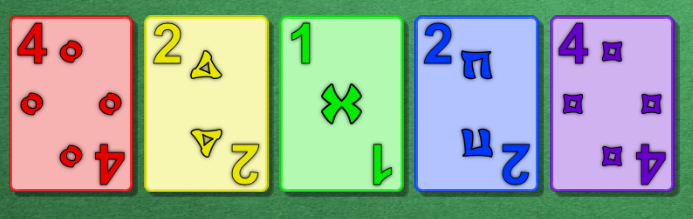
\includegraphics[width=0.5\columnwidth]{Figures/Hanabi Examples/example score area.png}
%     \caption{Hanabi Score area. In this example, the players scored 4+2+1+2+4=13 points.
%     %: 4 points from the red and purple colors, 2 points from the yellow and blue piles and 1 point from the green pile
%     }
%     \label{fig:example_score}
% \end{figure}



%In this section we detail the Hanabi domain in which we evaluated our learning scheme and the framework in which they were coded. Additionally, we provide a number of definitions for terms that will be used throughout this work.

% how hinting works
%The players may not talk freely to each other about what cards they are holding, but players may spend their turn to use the “Hint” action to provide information to another player.
Signalling in Hanabi happens implicitly through the play and discard actions, and explicitly through the players' hint actions.
In order to use a hint action, a player must   spend a hint token from a communal pool, which contains 8 tokens at the start of the game. Hints may be used to inform the other player about which cards in their hand have a single rank or color (e.g. ``these are the red cards in your hand''). All cards that share this property must be mentioned. An example of such communication is shown in Figure~\ref{hint example}.

\begin{figure}
     \centering
     \begin{subfigure}[b]{0.5\textwidth}
         \centering
         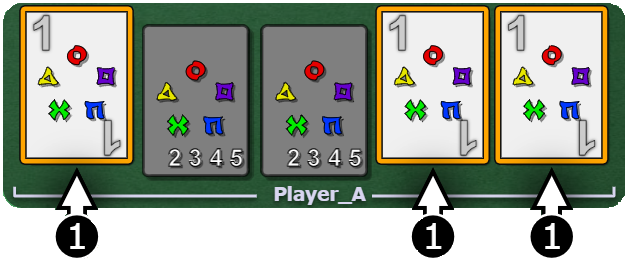
\includegraphics[width=\textwidth]{got hint.png}
       %  \caption{Player $i$ hand from their own point-ov-vie}
     \end{subfigure}
   %  \hfill
  %   \begin{subfigure}[b]{0.5\textwidth}
     %    \centering
     %    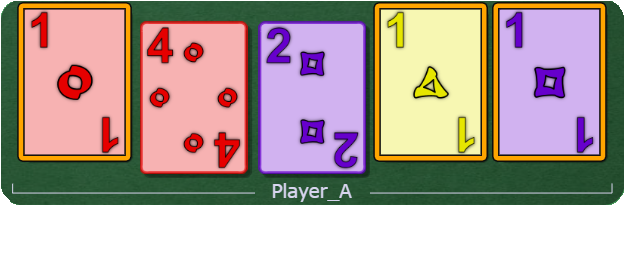
\includegraphics[width=\textwidth]{Figures/Hanabi Examples/actual hand.png}
      %   \caption{Player $i$ hand from player $(-i)$'s POV}
 %    \end{subfigure}
     \caption{A hand in Hanabi shown from the perspective of Player $A$ and a hint provided by the other player that reveals  that three cards (pointed to in the figure) have rank 1. Player $A$ can infer from the hint that  the other two cards are of ranks 2-5. The hint did not reveal any information  about the color of the cards, thus all five colors are possible.}
     \hfill
     \label{hint example}
\end{figure}

% how to regain hint tokens and the meaning of discarding cards
Players may also discard a card from their hand to return a hint token to the pool, which cannot contain more than 8 hints. All discarded cards are kept in a separate pile and are open information to all players. Discarded cards can't be played or returned to the deck or players' hands in any way.

% end conditions and scoring scheme
The game is over once one of the following conditions are met: (i) the players incurred 3 strikes; (ii) players cannot play a card with a greater rank than those already played; (iii) the cards in the  deck are depleted and each player has completed one turn.
% \begin{itemize}
%     \item
%     \item No card with greater rank than those already successfully played can be successfully played.
%     \item Each player had one turn since the deck has been depleted.
% \end{itemize}
Once the game is over, if the game did not end because of 3 strikes, then the score of the players is the sum of the highest ranks successfully played by the players in each color. The maximum score is the highest rank value times the  number of colors, which is 25.
% Figure~\ref{fig:example_score} shows an example of how the utility is computed.

% why we chose this domain
Hanabi is a fully cooperative game in which the channels of communication are limited and costly. It has been  shown~\cite{baffier2016hanabi} to be NP-Hard even with complete information.
Key to a successful strategy in the game is the ability to coordinate with one's partner by sending and receiving hints during the game.   It is thus  a popular domain for designing and
evaluating multi-agent strategies for cooperation and coordination~\cite{bard2020hanabi}.
%it a popular game for designing and evaluating agents. Thus, it is We are particularly interested in verifying whether humans are able to understand the hints and plays of an agent trained with our mixed-experience scheme.
%This makes conveying information difficult and requires the agents' strategies to consider the game state – and the previously observed actions – when interpreting a hint.
%Hanabi
%We chose this domain because an improvement in group score is directly tied to understanding other players' strategies.
We adapted the Hanabi Learning Environment for our experiments. We will make our code base publicly available after the conference's reviewing process.
%We make all of our code available for public use at the anonymous repository below.
%\footnote{A repository containing our code can be found here: \url{https://github.com/ecml233/Cooperative_RL_Agent_Hanabi}}.
% \footnote{\url{https://github.com/deepmind/hanabi-learning-environment}}.

% HLE~\cite{challenge} is an open-source environment that is written in Python and C++ and is simillar to OpenAI Gym~\cite{brockman2016openai}. The environment is used to test and produce consistent and reproducible results for all kinds of Hanabi playing agents. The environment is designed specifically with reinforcement learning agents in mind, with different regimes for evaluation suggested in the paper.


% \section{Problem Formulation}

% We consider the class of two-player partially-observable cooperative Markov games, which we define with a tuple $(S, I, O_i, A_i, U, T)$. Here, $S$ is the set of states, $I$ is the pair of players $(i, j)$, which we also refer as partners, $O$ is a functions that returns what player $i$ observes at a given state $s\in S$. $A_i$ is player's $i$'s set of actions, $U$ is a utility function that returns the  value for both $i$ and $j$ for a given action pair and state of the game (the game is fully cooperative), and $T$ is a stochastic transition function, that receives a state and an action pair, and returns the next state of the game. The goal of the players is to maximize their utility value.
\section{Methodology}


In Hanabi, RL-trained agents   perform well in self-play, achieving state-of-the-art performance, but have been shown not  to play well with humans~\cite{OP}.
 On the other hand, rule-based, deterministic strategies   are  better understood by  people  but such strategies are outperformed by RL agents in Hanabi. \kg{citation?}
 Our goal is to augment existing RL agents in Hanabi to be able collaborate both with human partners as well as other artificial agents. \kg{see earlier comment about framing goal}
To this end we wish to create Mixed-Experience Agents (MEA) by modifying the training regimes of existing RL agents to include interaction with  rule-based agents in addition to self-play. The rule-based agent   includes a set of    deterministic strategies  mapping states to actions in the game. %The strategies can be hand-crafted or selected from the literature.
 %We use a genetic programming approach to combine these hand-crafted rules  into a strategy~\cite{canaan2018evolving}.
 %The hand-crafted rules provided to the genetic programming approach try to capture the strategic knowledge of humans players and for that they tend to be more amenable to explainability.
 %were hand-crafted by players who tried to encode their domain knowledge into a set of useful rules, they tend to be more much more easy to understand.

 Prior work    has demonstrated that rule-based strategies are generally  interpretable, in that people are able to answer questions correctly about the decision boundaries  and write descriptions of such strategies successfully in different domains~\cite{lakkaraju2016interpretable}.  Thus we wish to verify whether RL agents are able to cooperate with people more effectively if trained with interpretable partners. Specifically we
 test the following hypothesis.
 \paragraph{}
 \emph{MEAs perform better with humans partners in Hanabi than  other RL agents trained  solely in self play. }
 \paragraph{}
% \kg{Levi, do you want to make the hypothesis more general?}
% \paragraph{Hypothesis 1:}
% MEAs perform better with humans partners in Hanabi than with other RL agents trained   in self play.

%We further hypothesize that MEAs  will also perform better when interacting in self-play  than  rule-based agents who interact in self-play.
%%removedVspace
%The rationale behind our hypothesis is that the experience generated from matches with a rule-based agent will bias the RL agent to be more amenable to collaboration with humans. This is because human players tend to quickly understand the logic behind the human-created rules used in rule-based systems. The RL algorithm will still be able to optimize the learned strategy to perform well in self-play (better than the rule-based agent used in training).


%\subsection{Learning Algorithm: Rainbow}

The steps in our methodology for evaluating the hypothesis are as follows. First, we choose a baseline  RL agent and an interpretable rule-based agent from the literature. % from the    RL literature and an interpretable rule-based agent from the game AI literature.
Second,
we train the baseline RL agent on  thousands of Hanabi games  using a mixed training regime that varies whether it interacts with the rule-based agent or in self play.
% Third, evaluate the augmented RL agent  by comparing its performance to  the baseline RL     and the rule-based agents in self-play on a set of new Hanabi games.
Lastly, we compare the performance of the MEA to the performance of the baseline RL agent and the rule-based agent when interacting with people. The remainder of this section describes the
first two steps in the methodology, while the next section describes a user study  that carries out  the  final step.

% We note that state-of-the-art Hanabi agents (2021) are computational costly to train, requiring  billions of training steps~\cite{op,SAD}.
\subsection{Agent Selection}
The   RL agent we  chose was DQN Rainbow~Hessel et al.~\shortcite{hessel2018rainbow},  which  is a domain independent multi-player RL agent using deep convolutional neural networks to approximate the action values for given states.
% making them perform We chose not to use the state-of-the-art algorithms we considered were SAD~\cite{SAD} and SAD with the Other Play enhancement (SAD+OP)~\cite{OP}. SAD+OP achieves higher scores than Rainbow and SAD in self play matches and it uses a domain-specific symmetry scheme that allows its learned strategies to perform well even with partner strategies they were not exposed to during training. The disadvantage of SAD and SAD+OP is their computational cost. While they require billions of training steps,

The rule-based agent was constructed from existing Hanabi agents using genetic programming,  following the approach by  Canaan et al.~\shortcite{canaan2018evolving}.  We began with an ordered  set of 50 deterministic rules   that was included in their code base,  and evolved  this rule set over 100 generations, evaluating fitness scores based on performance in self play.
After convergence, we reduced the size of the rule set  by  removing rules that were used in less than 1\% of a random set of 1,000 Hanabi games.  The resulting rule-based  strategy was represented as an  ordered list of 10 deterministic rules.  Representing the strategy as an ordered set assures  that identical states will always be assigned the same action by the strategy, without requiring that the rules themselves are consistent with each other.
%We verified that an agent using this rule set is   competent at the game, achieving an average self-play score of approximately 19 in self play.




% and it fails to achieve high scores when playing unseen interpretable partners. DQN Rainbow fails to achieve high scores with unseen partners because it learns unusual Hanabi game conventions that are not captured by existing rule-based strategies~\cite{canaan2020evaluating}. DQN Rainbow allows us to measure the degree in which our mixed-training scheme can bias the learned strategies toward strategies with which humans can effectively collaborate.

Other algorithms we considered were SAD~\cite{SAD} and SAD with the Other Play enhancement (SAD+OP)~\cite{OP}. SAD+OP achieves higher scores than Rainbow and SAD in self play matches and it uses a domain-specific symmetry scheme that allows its learned strategies to perform well even with partner strategies they were not exposed to during training. The disadvantage of SAD and SAD+OP is their computational cost. While they require billions of training steps, DQN Rainbow requires only millions of training steps. Since we foresaw training multiple versions of the agent to test different training mixture regimes, we chose to use DQN Rainbow. Moreover, we wanted to measure the effect of mixed-training in the agent's ability of cooperating with humans. The domain-specific enhancements implemented in SAD+OP would not allow us to measure the effect of mixed training in isolation.
%Nevertheless, evaluating mixed-training schema with SAD+OP is a research direction that is worth investigating.


%substantially more computational resources than Rainbow, we decided to experiment with the latter.


\subsection{A Mixed Training Regime}
\label{training regimes}
A training regime determines  for a given Hanabi game whether the RL agent  is interacting with  an agent using  a rule-based strategy or in self-play mode. An epoch is defined as 10,000 steps (actions) in Hanabi, which can span several games. All agents were trained for a total of  10,000 epochs.  This is the same number of steps used by Bard et al.~\shortcite{bard2020hanabi}.




For purposes of comparison,  we  show the performance of the Baseline Rainbow agent of Hessel et al.~\shortcite{hessel2018rainbow} as a function of the number of epochs used in a traditional RL training regime. Performance is computed at the end of each training epoch as the score of the Baseline Rainbow agent in self-play mode as well as  when interacting with the rule-based agent for 1,000 random Hanabi games.

Figure~\ref{fig:performance} (top) shows the mean score of the Baseline Rainbow agent in self-play mode  (blue curve) and  with the rule-based agent (green curve). The red curve corresponds to the rule-based agent's self-play score, which does not change over time. Curves in the figure show a moving average of 10 epochs;  the  shaded area  surrounding the curves shows the corresponding standard deviation.
% of the 1,000 games played.

%We show  the performance of the Baseline Rainbow in self-play   (blue curve) and  with the
%rule-based agent (green curve).
% The mean scores are computed using a moving moving average of 10 epochs;  the  shaded area  surrounding the curve show the  corresponding standard deviation of the 1,000 games played.
\begin{figure}[t]
    \centering
    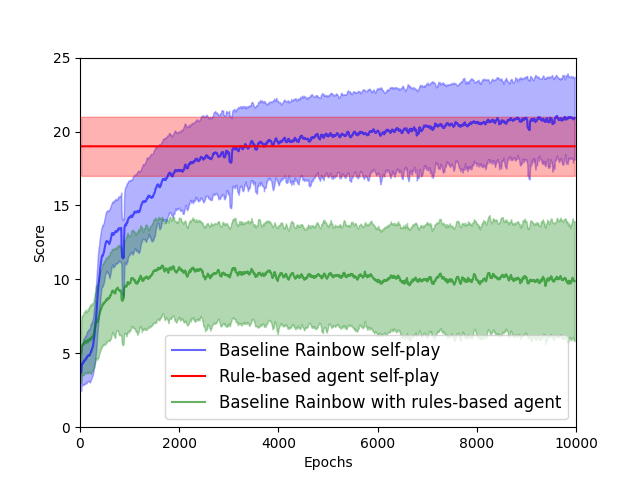
\includegraphics[width=8cm]{baseline.png}
    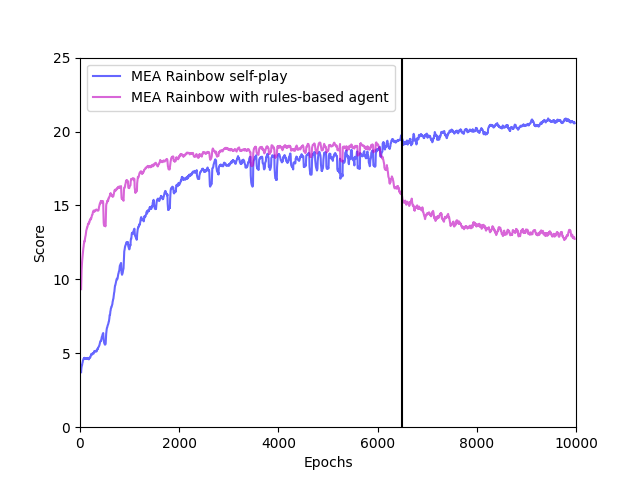
\includegraphics[width=8cm]{mixed.png}
    \caption{Baseline Rainbow (top) and MEA  Rainbow (bottom)   performance as a function of training   epochs. Shaded areas represent standard deviations. The black vertical line represents the number of epochs used to train the MEA agent selected for the user study.
    % The means are surrounded by colored areas which represent the corresponding standard deviations.
    }
    \label{fig:performance}
\end{figure}

As shown by the plot, the Rainbow agent quickly increases its self-play score, with the rate of improvement slowing over time, plateauing at a self-play score of about 21. Its performance  with the rule-based agent also begins by increasing for about 2,000 epochs,   from a score 5   and plateaus at a score of 10.
% We also included the score of the rule-based agent in self-play (red curve), which is constant
% across the training epochs.


We propose to modify the traditional training regime to vary whether the Rainbow agent interacts in self-play or with the rule-based agent for a given number of epochs. In this new \emph{mixed} regime, Rainbow alternates between training in self-play for the first  $n_1$ epochs, then training with the  rule-based agent for  another $n_2$ epochs, and repeats this process $k$ times.  For the remaining number of epochs (set to a constant 40\% in this work), Rainbow trains solely in self-play mode.
%The resulting MEA Rainbow agent is subsequently evaluated
%on a random set of 1,000 Hanabi games.
%the first $p$   percent of the   training epochs.
% We experimented with different  values of $n_1$ and $n_2$ (Figure~\ref{fig:training regimes illustrations} (b) shows a Mixed regime with $n_1=n_2=1$, $p=60$).
%For the remaining $100-p$ percent of epochs, Rainbow is trained solely in self-play.
Figure~\ref{fig:training regimes illustrations}  shows a mixed regime   with configurations  $n_1=n_2=1$ (left) and $n_1=2$, $n_2=1$ (right).
%In this work, we only tested configurations with different values of $n_1$.

% In the \emph{Rules Priming} regime,   Rainbow interacted   with a rule-based agent for the first half of  the training epochs, followed by training solely in self-play for the second half of the training epochs.
% In the \emph{Mixed} regime,   Rainbow alternated between training in self-play for $n_1$ epochs, then training with the  rule-based agent for $n_2$ epochs for the first $p$   percent of the   training epochs. We experimented with different  values of $n_1$ and $n_2$ (Figure~\ref{fig:training regimes illustrations} (b) shows a Mixed regime with $n_1=n_2=1$, $p=60$). For the remaining $100-p$ percent of epochs, Rainbow was trained solely in self-play.
%This was done with the intention of increasing its self-play score to be comparable with a regularly trained Rainbow. For the first part of training, where training types where mixed,
% Lastly, in the \emph{3-Phase} regime,
%In this form of training, we wanted to explore if priming Rainbow by playing solely in self-play can benefit the Mixed Training regime.
% Rainbow was first trained for $p_1$ percent of its total training epochs solely in self-play.  For the following $p_2$ percent of training epochs, Rainbow alternated between training in self-play  for $n_1$ epochs, then training with   the rule-based agent for $n_2$ epochs. For the remaining $100-p_1-p_2$ percent of epochs, Rainbow was trained solely in self-play. \kg{missing some logic here...}

\begin{figure}[t]
\centering
         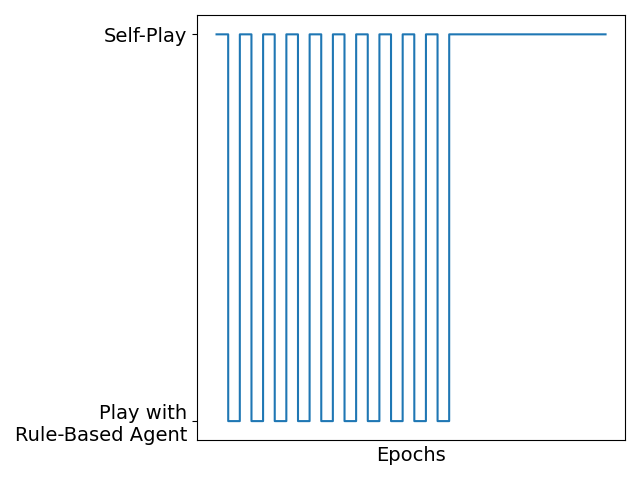
\includegraphics[width=3.5cm]{mixed illustration n=1.png}
         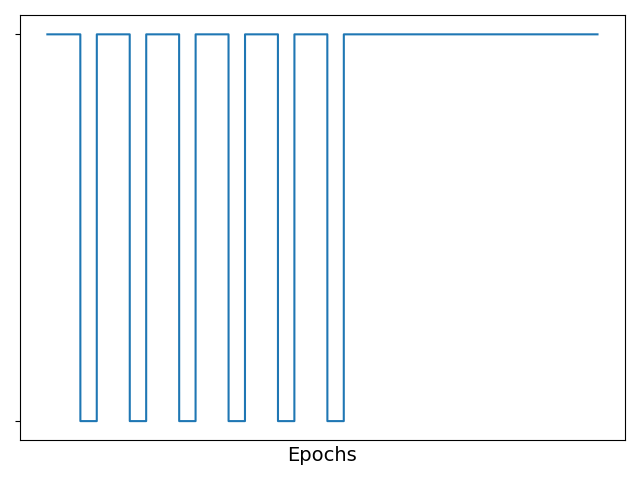
\includegraphics[width=3.5cm]{mixed illustration n=2.png}
         \caption{Illustrations of our mixed training regime configured  with $n_1=n_2=1$, $k=3,000$ (left), and $n_1 = 2$, $n_2=1$, $k=2,000$ (right). Length of $x$ axis is  not to-scale}
                           \label{fig:training regimes illustrations}
\end{figure}

% \begin{figure}[t]
% \centering
%          \includegraphics[width=4.00cm]{Figures/Modified training/regime visualization/rules priming epochs.png}
%                   \includegraphics[width=4.00cm]{Figures/Modified training/regime visualization/mixed regime epochs.png}
%          \includegraphics[width=4.00cm]{Figures/Modified training/regime visualization/three part regime epochs.png}
%          \caption{Illustrations of   Rules Priming regime (left), Mixed regime (middle), and 3-Phase regime (left). Training times are not to-scale}
%                           \label{fig:training regimes illustrations}
% \end{figure}


% \subsection{Training Regime Evaluation}

% In this section, we present the results of the both the offline evaluations and user study we conducted to evaluate the proposed approach. Figures in this section show a moving average (window size of 10), with means surrounded by a shaded area which represents the corresponding standard deviation.
% \subsection{Training Evaluations}

%\subsection{Evaluation}


 Figure \ref{fig:performance} (bottom) shows the performance of an MEA Rainbow  as a function of training time for the   configuration of the  mixed training regime that yielded best performance ($n_1=n_2=1$).
Performance is computed at the end of each training epoch as the score of the MEA Rainbow agent  in self-play mode  (blue curve) as well as  when interacting with the rule-based agent (green curve) for 1,000 Hanabi games.
As before, each point in the plot represents a  sliding window of size 10. We remove the shaded areas representing standard deviations in score to improve readability; standard deviation for these curves are similar to those presented in the plot at the top of   Figure \ref{fig:performance}.
%  As seen in the figure,
 %the mixed regime allows the performance of the MEA Rainbow to improve, both in terms of its self-play score, as we as when interacting with the rule-based agent.
As shown in the figure, for the initial 60\% of epochs, the performance of the MEA Rainbow monotonically increases in terms of its self-play score, as well as when interacting with the rule-based agent.
The performance plateaus at about the same score as that of the rule-based agent in self-play, with
the score of MEA Rainbow in self play being slightly smaller than the score of Baseline Rainbow in self play.
In the last 40\% of epochs, when MEA Rainbow trains solely in self play, we see a monotonic decrease in its score with the rule-based agent, that plateaus slightly higher than the score of  Baseline Rainbow playing with the rule-based agent (see plot at the top). At the same time, the score of the  MEA Rainbow in self play monotonically increases and reaches that of Baseline Rainbow.

%At the point in the regime when training switched to be solely in self-play (\kg{when is that?}, the self-play score converges with that of the Baseline Rainbow and the score with the rule-based agent quickly decreases.

The black vertical line in Figure \ref{fig:performance} (bottom) represents the period in the training regime  after 6,500 epochs, 500 epochs after the MEA Rainbow agent switched to training solely in self play.
To see why this point represents an interesting tradeoff in the training regime, we present
%At this point, the   MAE Rainbow score in self play (blue curve, right) is greater than the rule-based agent score (red curve, left). At the same time, the  MAE Rainbow score when interacting with  the rule-based agent (green curve, right) is significantly higher    than that of the Baseline Rainbow agent interacting with the rule-based agent (green curve, left).
%  We used an agent which was trained for 6,500 epochs, as designated by the black vertical line shown in  Figure \ref{fig:performance} (right).
 Figure~\ref{fig:bar_plot}, which  compares  the performance of the MEA agent at the 6,500 epoch point to that of the Baseline Rainbow and rule-based agent.
    This point in the training regime is a `sweet spot' which satisfies the following criteria: The performance of  MEA Rainbow when interacting with the rule-based agent significantly outperforms the Baseline Rainbow agent  (15.37 compared to 10.28, $p < .05$ using Mann-Whitney test)
    %, U=3858235, p$<$1e-36)
    while its performance in self-play is already statistically significantly higher than that of the rule-based agent (19.66 compared to 19.13,  $p < .05$ using Mann-Whitney test).
    %, U=10672313.0, p$<$1e-36).
    Following these results, for the user study, we selected the MEA Rainbow agent which was trained for 6,500 epochs in the $n_1=n_2=1$ configuration.

    %By choosing different stopping points on the x-axis of Figure~\ref{fig:performance} (bottom) we can obtain agents with different skill levels in self-play games and in games played with the rule-based agent.
    The learning curves shown in Figure~\ref{fig:performance} (bottom) suggest that we obtain an agent with performance similar to the rule based agent if we stop training immediately before training solely in self play. Moreover, this agent plays equally well in self play and with the rule-based agent. If we continue training long enough in self play, then we obtain an agent with performance similar to the Baseline Rainbow and that performs better in self play than with the rule-based agent. If we stop training anywhere in between these two extremes we obtain an algorithm that trades off self play score with the score obtained in matches with the rule-based agent. %The score with the rule-based agent act as a proxy for interpretability and for how well the agent cooperates with humans.
    Under the assumption that the score with the rule-based agent offers a proxy to how well the agent cooperates with humans, the number of training epochs of self play after the mixed regime allows us to design agents that vary their ability to cooperate with humans from ``similar to the rule-based agent'' to ``similar to Baseline Rainbow.''

   %Following these results, for the user study, we chose the   MEA agent which trained for 6,500 epochs.
    %.  In such experiments, Rainbow's self-play score increased and its score with the rule-based agent deceased when skewing the ratio in favour of self-play.
% In all cases, the self-play score is always worse than that of the rule-based agent, so we are less interested in those.





    \begin{figure}[t]
    \centering
    \includegraphics[width=7.0cm]{bar plot.png}
    \caption{Mean scores of Baseline Rainbow, MEA Rainbow and rule-based agent over 5,000 Hanabi games. Black lines on bars represent the corresponding standard deviation\kg{it's too small}}
    \label{fig:bar_plot}
\end{figure}
% We now show the results of the last suggested training regime - 3-Phase. Figure \ref{fig:3-phsae} shows the scores generated when $n_1=n_2=1$, $p_1=30$, and $p_2=50$.
% % the first phase is completed with only self-play training and the mixing ratio of the second phase is 1:1.
% We see that the first phase is the same as the baseline, and the second phase resembles that found by using only the Mixed regime. As before, when starting the final phase, training solely in self-play, the score in self-play converges with that of the baseline, and the score with the rule-based agent decreases rapidly.

%We also evaluated this regime with other greater values for $n_1$.
%\uf{we're saying something very similar to what we said in the above paragraph here.}

%This value was chosen as it still resulted in the highest score when playing with the rule-based agent among the tested values, while retaining a self-play score which is higher than that of the rule-based agent's.

\begin{figure}[t]
\centering
        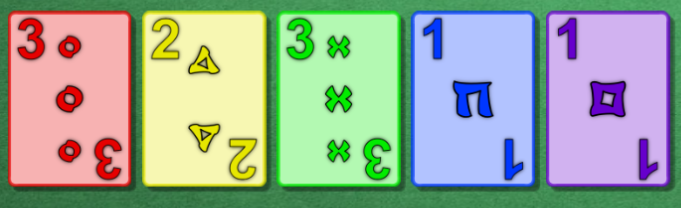
\includegraphics[width=4.50cm]{cards already succefuly played.png}
        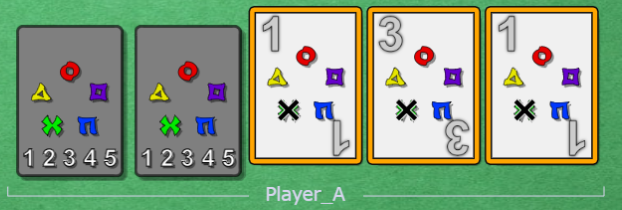
\includegraphics[width=4.50cm]{hand prior to hint.png}
        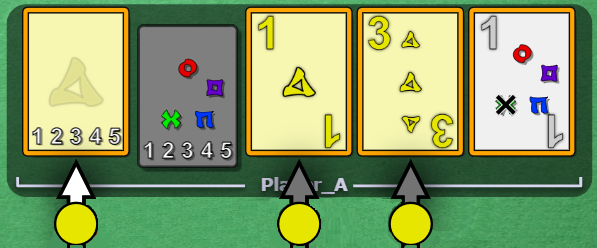
\includegraphics[width=4.50cm]{hand knowledge after hint.png}
\caption{Example illustrating the difference  between baseline and MEA Rainbow in a representative state of a Hanabi game. The top row shows the cards played in the game, the middle row shows the player's knowledge about their own hand, the bottom row shows a hint MEA Rainbow gave.}
                           \label{fig:agents_example_comparison}
\end{figure}

We end this section with an illustrative example of how the strategy of the MEA Rainbow is more amenable for cooperation with people than that of the  Baseline Rainbow.
%We played a game of Hanabi with the baseline agent and logged states where its actions seemed unintuitive. We then quarried MEA Rainbow for its actions in those states and compared the two. MEA Rainbow's action seemed more explicable than those of the baseline.
%Consider an intermediate state in a Hanabi game in which
Figure~\ref{fig:agents_example_comparison} (top) shows the cards that were played at an intermediate state of a given Hanabi game.  A player's knowledge of its own hand at this state is shown in Figure~\ref{fig:agents_example_comparison} (middle).
The player can infer that both of its rank 1 cards are useless, because all rank 1 cards of all colors have already been successfully played.  In this state, the  Baseline Rainbow generated a hint to the player   about their rank 1 cards. This hint provides no  valuable information to people who are unaware of the strategy of Baseline Rainbow.
%to someone who is not aware the cryptic convention of play that is being communicated with this particular hint.
In contrast, MEA Rainbow generates a  hint about  our yellow cards in this state, providing valuable and easy-to-understand information about 3 cards; see Figure \ref{fig:agents_example_comparison} (bottom).
%Note that in self-play mode, the Baseline Rainbow agent gives back a hint




% We don't present plots for the other values of $n_1$, $n_2$, and $p$ we tested. In such experiments, the self-play score increased and the score with the rule-based agent deceased when skewing the ratio in favour of self-play, and vice-versa.  \uf{A question that might come up is why not use p=0.95 instead of shortening the total training time for the agent we ended up using for the user trial}



\section{User Study}
In order to evaluate our hypothesis we conducted a user study in which participants played Hanabi games
with three types of agents: (1) The rule-based agent that was used as a training partner for Rainbow; (2) the Baseline Rainbow agent of Hessel et al.~\cite{hessel2018rainbow}; (3) a MEA Rainbow agent which was trained in the mixed regime with $n_1=n_2=1$, trained on 6,500 epochs.
%     The score achieved by this agent is designated by the black vertical line shown in  Figure \ref{fig:performance} (right). This point  in the training regime is a `sweet spot' which satisfies the following criteria: The performance of  MEA Rainbow when interacting with the rule-based agent significantly outperforms the Baseline Rainbow agent  (15.37 compared to 10.28, using Mann-Whitney test, U=3858235, p=0) while its performance in self-play is still statistically significantly higher than that of the rule-based agent (19.66 compared to 19.13,   using Mann-Whitney test, U=10672313.0,p $<$ 1e-36). \kg{mention criteria.}


%     \begin{figure}
%     \centering
%     \includegraphics[scale=0.5]{Figures/bar plot.png}
%     \caption{Mean scores of Baseline Rainbow, MEA Rainbow and rule-based agent over 5000 games. Black lines on bars represent the corresponding standard deviation}
%     \label{fig:bar_plot}
% \end{figure}

    %We had each agent play 5000 games in self-play, both using the same string of decks. A Mann-Whitney test on a the results indicated that the self-play scores of Augmented Rainbow are greater than those of the rule-based agent, U=10672313.0, p $<$ 1e-36. We also calculated the effect size to be ~0.153 (Cohen's d). Additionally, The augmented agent had achieved a perfect score 4.8 times more often than the rule-based agent.

    %The agent was not trained for the full duration, and only had 0.05e8 training steps in self-play, as opposed to the usual 0.4e8. Its scores can be seen in Figure \ref{fig:regime_evals} (middle), as it is a snapshot of that agent after 0.65e8 training steps (marked with a black vertical line).

% For the third agent, We chose to use this version of Rainbow for the user study as it has a higher self-play score than the rule-based agent (19.66 compared to 19.13), and its score with the rule-based agent is much greater than the baseline (15.37 compared to 10.28).

% Because of the high variance in the scores of agents, we verified that the MEA Rainbow is better than the rule-based agent in self-play by playing another string of games.


% Because of the high variance in the scores of agents, we verified that the difference in score of this agent and the rule-based agent in the self-play setting is significant. We had each agent play 5000 games in self-play, both using the same string of decks. A Mann-Whitney test on the scores returned a p-value < 1e-36 and calculated that Cohen's-D is ~0.153.

% While versions of Rainbow which were trained using the Rule-Priming regime achieved comparable scores during their training, agents trained using the Mixed regime showed lower variance in score.

% While training this agent longer in self-play improves its self-play score, it would also greatly decrease its score with the rule-based agent. Even though the scores of the agent are comparable to those of the in score than the agent which was trained using the Rules-Priming regime.

% consdier where to put this

%We also hypothesised that users will perform much worse with the Baseline Rainbow, as there are plenty of examples\cite{chattopadhyay2017evaluating,OP} that show that it is usually hard for humans to cooperate with RL agents. Finally, we hypothesised

The study, which was approved by the IRB of the relevant institution, was conducted through Amazon Mechanical Turk and included 83 participants. All participants had little experience playing board games and no experience playing Hanabi.

\subsection{Study Design and Results}
Each participant was randomly paired with one of the agents and was asked to play a series of games with that agent  using an online  platform for Hanabi (\url{hanab.live}) that we configured for our experiment.  Participants were told they would be playing with a computer agent, but  received no explanation about how it was designed, or about its strategy. They were allowed to drop out of the study at any point. Participants received a constant show-up fee of \$0.4 and paid by performance in the games up to \$30.  %After participants completed their game, they were asked to fill out a short survey about their experience.
% \begin{figure}
%     \centering
%     \includegraphics[width=0.7\columnwidth]{Figures/hanab live example.png}
%     \caption{Example of the game interface in hanab.live}
%     \label{fig:example_interface}
% \end{figure}
% After completing their first game, participants answered both demographic questions and questions about how well the users felt they understood the agent they played with.
We also asked participants  questions about their subjective opinion of the quality of the agent's strategy. Specifically, we asked  how they enjoyed playing with the agent and how the agent responded to their hints. Participants could also provide (optional) written statements about their experience.
%Participants were asked to rank how well they thought the agent played Hanabi using a 5 point Likert scale.

% Besides the users self-reported understanding, we also measured the average score that each type of agent scored. We looked at the scores of the first games players played with agents, and the scores of all games played with each agent.

In total 265 Hanabi games were played,  evenly divided among the three different types of agents.
Each participant played (on average) approximately 3 games of Hanabi.
Following our hypothesis, we  expected that users will be able to perform better with MEA Rainbow than with the Baseline Rainbow agent. We also expected that the rule-based agent will achieve the best performance with people,  as its strategy is comprised of a short list of   interpretable rules.

Table \ref{user_results} shows the main results of the study for the rule-based agent (``Rule-Based''), MEA Rainbow (``MEA''), and Baseline Rainbow (``Baseline''). %As shown in the table, people performed best with the rule-based agent, followed by the MEA agent. The  worst agent was the baseline version of Rainbow.
% We can see a significant difference both in the average score of users' first games, as well as the average score overall.
We show performance in the game (average score), as well as the average Lenient score, which refers to the highest score obtained by people, disregarding strikeout, as was used by Hu et al.~\cite{OP}.
\kg{suggest to move the line below 598 to the end of the paragraph and to include a short discussion about the benefits of MEA when there is uncertainty about the identity of the other agent.}
The rule-based agent achieved the best results in our user study, with the highest average score, highest average lenient score, and  lowest strikeout rate. MEA Rainbow achieved the second best results, followed by the baseline Rainbow agent.
Participants playing with MEA Rainbow achieved more than three times the average score obtained by the participants playing the Baseline Rainbow. The difference in score is also large for the lenient scoring scheme: The score obtained by the participants playing with MEA Rainbow was more than twice that obtained by the participants playing Baseline Rainbow. The larger gap in terms of regular score between MEA Rainbow and Baseline Rainbow is due to a larger strikeout rate of Baseline Rainbow. Many of the games played between the participants and Baseline Rainbow finish with the players achieving the third strike due to miscommunication of which cards should be played.

\begin{table}[t]
\uf{Added lenient score to table, an explanation about it in caption}
% \setlength{\tabcolsep}{5pt}
\footnotesize
\centering
\begin{tabular}{ l c c c }
    %p{0.35\textwidth}|p{0.15\textwidth}|p{0.225\textwidth}|p{0.225\textwidth}|}
 \toprule
  & Rule-Based &  MEA & Baseline\\
 \midrule
 Number of Participants & 25 & 30 & 28 \\
 Number of Games Played & 80 & 92 & 93 \\
 %\hline
 %Avg. num. games per user & 3.2 & 3.01 & 3.32 \\
 %Average score in first game & 9.6 & 6.2 & 0.82 \\
 %\hline
 Average Score & ${8.82}$ & 6.18 & 1.77 \\ [1ex]
 Average Lenient Score & $\bf{11.45}$ & 9.2 & 4.26 \\ [1ex]
 Average Strikeout Rate & 0.45 & 0.56 & 0.76 \\
 \bottomrule
\end{tabular}
    \caption{User study  results.
    Participants performed best with the rule-based agent, closely followed MEA Rainbow, and worst with Baseline Rainbow. }
\label{user_results}
\end{table}
% There was a statistically significant difference between the first games score and totals scores of all three groups (H$\approx$15.59, p$\approx$0.0004 and H$\approx$30.526, p$\approx$2.35e-07, respectively). A Mann-Whitney test on a the first games score and totals scores indicated that those of MEA Rainbow are greater than those of Baseline Rainbow, U=281.5, p$\approx$0.0026 and U=3131.0, p$\approx$5.378e-05, respectively. The effect sizes of first games scores and total scores for these agents are 0.3676711 and 0.2848589, respectively.
There was a statistically significant difference between the average scores of all three groups %(H$\approx$30.526, p$\approx$2.35e-07).
($p < .05$).
A Mann-Whitney test indicated that the average score of people playing with MEA Rainbow (6.18) is greater than those of the people playing with Baseline Rainbow (1.77) ($p < .05$).
% U=3131.0, p$
% \approx$5.378e-05.
The statistical tests point to a medium effect sizes of average scores: $0.28$.
These
results
support our hypothesis.

We also look at the strikeout rates, which are instances when players incur 3 strikes, immediately ending the game with a score of 0, if using the non-lenient score scheme. The strikeout rate offers a good proxy of how well people understood the strategy played by their  partner. This is because players need to minimize non-successful plays (strikes), which usually happen due to miscommunication between the players. Therefore lower strikeout rates mean that miscommunications between the players happened less often than in games with higher strikeout rates.
%There was a statistically significant difference between the   strikeout rates of all three groups (H$\approx$8.642, p$\approx0.013$), showing .
A Mann-Whitney test indicated that the strikeout rates of the Baseline Rainbow (mean 0.76) are higher than those of MEA Rainbow (mean 0.56), with $p < .05$. The effect size was $0.23$, which is medium to small.
%, U=310, p$\approx$0.035. The effect size is 0.2389121.

% Our version of Rainbow scores slightly less than the rule-based agent, and significantly more than regular Rainbow.
% Kruskal-Wallis tests on the first games scores and total scores of all 3 groups returned P values of 0.0004 and 2.35e-07, respectively. Mann-Whitney tests on the first games scores and total scores of the Baseline Rainbow and tested Rainbow return P values of 0.002 and 5.37e-05, respectively. The effect sizes of first games scores and total scores are  0.3676711 and  0.2848589, respectively.

% Additionally, we look at the strikeout rates - instances when players incur 3 strikes, immediately ending the game with a score of 0. This happens significantly more often with regular Rainbow than with the rule-based agent. As before, our version of Rainbow struck out more often than the rule-based agent, but significantly less than regular Rainbow.
% Kruskal-Wallis tests on the strikeout rates of all 3 groups returned P values of 0.013, and Mann-Whitney tests on the strikeout rates of the Baseline Rainbow and tested Rainbow return P values of 0.035. The effect size is 0.2389121.

\subsection{Survey Results}

% TODO mention that these results are not statistically significant
\begin{table*}[t]
\centering
\footnotesize
    \begin{tabular}{c p{0.45\textwidth}ccc}
 \toprule
 \# & Question & Rule-Based & MEA & Baseline \\ [0.5ex]
 \midrule
1 & How well did you understand the AI's strategy?  & 3.08 & 2.87 & 2.39 \\
\midrule
2 & How well does the AI play Hanabi? & 3.44 & 3.01 & 2.71 \\
\midrule
3 & How much did you enjoy playing with the AI?   & 3.56 & 3.23 & 2.96 \\
 \midrule
4 & How often did the AI respond to your hints as you intended? & 3.36 & 2.70 & 2.61 \\
 \midrule
5 & How often did you think you responded to a hint given to you by the AI as it intended? & 3.48 & 3.53 & 3.21 \\ [1ex]
 \bottomrule
\end{tabular}
\caption{User study survey.
    Users ranked the rule-based agent as most understandable, closely followed by MEA Rainbow, and finally Baseline Rainbow as the least understandable.}
    \label{survey_table}
\end{table*}

After playing the games with their artificial partner, each participant answered a survey about their experiment playing the agent.
%This result was supported by a survey we conducted with the participants in the study which
%asked them
We asked the participants
to rate their experience when interacting with the different agents.
Table \ref{survey_table} shows the survey questions posed to participants and their responses on a Likert scale between 1 and 5, where 1 is a negative answer and 5 a positive one. We number the questions from 1 to 5 (see leftmost column).  Users' perceptions about the agents' strategies generally aligned with the results presented in Table~\ref{user_results}, in that  users ranked the rule-based agent as most understandable, closely followed by MEA Rainbow, and finally Baseline Rainbow as the least understandable. The same ordering is also true for the users' evaluations of how well the agent plays Hanabi and their enjoyment of playing with them.
We note that although the trends are clear, we did not find statistically significant differences in the  Likert scores reported. % in  the 3 groups.
%On average, users rated their understanding of the agent's strategy highest for the rule-based agent, followed closely by MEA Rainbow, and finally Baseline Rainbow.

An interesting aspect of the survey refers to Questions 4 and 5.
When asked to rank how often the agent reacted to their hint as they intended (Question 4), the rule-based agent was ranked highest of the three with an average of 3.36, with MEA coming in second with an average of 2.70 and Baseline Rainbow in third with 2.61. %, but both versions of Rainbow were ranked    lower than the rule-based agent.
%Based on  users' responses, it seems that this is mostly due to a specific kind of miscommunication. Once a user has provided the agent with complete information about a playable card in their hand and the agent fails to play it, users might become frustrated with their interaction with the agent and cooperation becomes much harder to accomplish.
When asked  how often participants thought that they responded correctly to a hint given to them by the artificial agent (question 5), MEA was ranked slightly higher than the rule-based agent, with an average of 3.53 compared to 3.48. The lowest was Baseline Rainbow with 3.21.
The results for Questions 4 and 5 suggest that users felt they understood the  hints from artificial agents more than the agents understood their own hints. This is likely because there are different ways to interpret a hint from a player, while one usually has a specific goal in mind when providing a hint to their partner.

% One explanation for the discrepancy in scores for questions 4 and 5 for the MEA Rainbow agent is due to a discrepancy in the skill level of the participants and of the MEA agent. The MEA agent might be able to choose a better action than the action the participant had expected it to play. While question 5 can also have effects related to skill discrepancy, the fact that the participants answered question 5 positively
% %mostly agree that they responded to the hints provided of the MEA agent as it intended
% indicates that the hints the MEA agent provided were comprehended by the participants.
% %could leave the participant with the impression that the MEA agent did not



\subsection{Discussion}

The results of the user study supported our hypothesis, in that the MEA Rainbow achieved significantly better performance when interacting
with people than Baseline Rainbow.
The results also confirmed that the rule-based agent was able to achieve a reasonable level of cooperation with inexperienced human players.  In contrast, the Baseline Rainbow was unable to cooperate well with humans, likely due to the specific strategy conventions learned in the RL training regime.
% We do not
%This aligns with previous work demonstrating the  benefit of rule-based strategies in other domains~\cite{lakkaraju2016interpretable}.

%The participants agreed less often that they had understood what the Baseline Rainbow agent intended with its hints.
%Understanding the hints provided by the player's partner is essential to achieve high scores in the game.

%The results obtained with Baseline Rainbow are also in line with results presented in previous works, which showed that Baseline Rainbow is unable to cooperate well with artificial agents trained with other algorithms (e.g., rule-based agents)~\cite{canaan2020evaluating}.
%Here, we showed that

The MEA training scheme allowed the RL agent to learn effective strategies for cooperating with humans in Hanabi at the cost a reduced score in self-play matches. MEA Rainbow is able to train agents that fall in between rule-based agents and regular RL agents in terms of self-play strength and ability to cooperate with humans. The MEA Rainbow agent is significantly stronger than the rule-based agent in self play matches, but not as effective as the rule-based agent while cooperating with humans. The MEA Rainbow is significantly more effective while cooperating with humans than the Baseline Rainbow, but not as effective as Baseline Rainbow in self play matches.
This reflects   the  performance tradeoff  of the augmented RL regime that was observed in training (Figure~\ref{fig:training regimes illustrations}),  in that   MEA   performed better with people than the baseline RL agent, but worse than the rule-based agent.
The MEA is ideal for settings in which the identity (human or agent) of the partners is unknown.

A possible reason for the success of the MEA agent is that it  effectively biases the search performed by the RL algorithm in the strategy space to a region where the strategies are more amenable to interpretability, i.e., strategies more similar to rule-based strategies. Intuitively, when we switch from mixed-experience training to self-play training (see Figure~\ref{fig:performance}), the agent is capable of learning non-interpretable strategies, similar to those Baseline Rainbow learns, after a sufficiently large number of steps. Unfortunately this comes at the price of forgetting how to play the game with the rule-based agent, as can be observed in Figure~\ref{fig:performance}. This may be  related to the issue of catastrophic forgetting in machine learning, where trained models forget previous connections after learning new ones~\cite{mccloskey:catastrophic}. As shown in our user study, a model trained with only a limited amount of only self-play experience is still able to cooperate well with humans while achieving high scores in self-play.



The  survey results show a trend  that also supports our hypothesis. This is because the participants reported they  understood the signals of the MEA agent more than those of the Baseline Rainbow agent. %, which is a crucial element in successful Hanabi play.
%. The limited number of self-play training steps we can perform before the  learned strategy becomes hard to understand limits how much better the MEA agents are in comparison to rule-based agents.


%after a limited number of training steps the agent might still be playing an interpretable strategy that favors cooperation with humans while achieving higher scores in self play.

%simply optimize the interpretable strategy it learned to play with the rule-based agent. The results of our user study suggest that the self-play experience generated after training with the rule-based agent allows

%Move to conclusions?
%Our approach was domain agnostic, in that we took a general RL agent and augmented its strategy to cooperate with people in a given setting. Our only requirement is the existence of a rule-based strategy for the domain which is possible to be taken from the literature or constructed with synthesis methods, as we did in our experiments. % (e.g., with genetic programming).

%Most importantly, our results fully support Hypothesis 1 as MEA Rainbow achieved significantly higher scores while playing with humans than Baseline Rainbow. Moreover, our trained MEA agent also satisfies the requirement that it is able to achieve higher scores in self play than the rule-based agent.

%also confirmed the results of previous works that showed that Baseline Rainbow learns conventions are too specific to the trained agents and does not generalize to other agents trained  (i.e., it is unable to cooperate with other agents)




% Details of the demographic data of participants can be seen in table \ref{demo_table}.
% % The test group had a larger percentage of females, however, the average score of females was lower than that of males in all three groups.

% \begin{table}
% \centering
%     \caption{Demographic results.
%     No significant difference between the three groups.}
%     \begin{tabular}{p{0.4\textwidth}p{0.15\textwidth}p{0.15\textwidth}p{0.15\textwidth}}
%  \hline
%   & Rule-Based Agent & Regular Rainbow & 2-Phase Trained Rainbow \\ [0.5ex]
%  \hline\hline
%  What is your gender? (0: male, 1: female) & 0.12 & 0.21 & 0.43 \\
%  \hline
%  How old are you?  & 29.4 & 32.75 & 34.17 \\
%  \hline
%  How much experience do you have playing board games? (0 is least experience) & 1.52 & 1.53 & 1.63 \\
%  \hline
%  How much experience do you have playing Hanabi?  (0 is least experience)  & 0.16 & 0.21 & 0.23 \\
%  \hline
%  When was the last time you played Hanabi before today?  (0 is least recent) & 0.24 & 0.32 & 0.53 \\[1ex]
%  \hline
% \end{tabular}

%     \label{demo_table}
% \end{table}

\section{Conclusions}



% \section{Conclusions}
% Through the usage of modern techniques, AI agents are able to achieve amazing results in various tasks. Some of these tasks require cooperation with other agents. Ad-hoc cooperation remains challenging for most agents, and especially cooperation with humans.

 %In this work, we presented an approach that aims to

% reduce the difficulty of such cooperation. It tried to accomplish this by making a given RL agent easier for people to perform well with.

% We end this section with a short discussion of  limitations of the work.

This paper presented a new approach for designing RL agents for interacting with people in two-player cooperative games.
%We have shown that DQN Rainbow is able to learn strategies that cooperate well with humans by exposing the RL learner to rule-based strategies during training. We showed that the RL agent can be exposed by interweaving self-play experience with experience produced in matches with a rule-based agent.
%We presented how various changes to RL agents' training regime can affect their performance with rule-based strategies. We've shown that exposing an RL agent to other strategies during its training must be interwoven into self-play training steps.
%as otherwise the RL agent quickly reverts to the same strategy created in self-play only training.
We explored the trade-off between performance in self play and performance with a rule-based strategy. Our approach is domain agnostic, in that we took a general RL agent and augmented its strategy to cooperate with people in a given setting. Our only requirement is the existence of a rule-based and interpretable strategy for the domain. % which is possible to be taken from the literature, or constructed (e.g., with genetic programming).
We presented a way to train RL agents so that their high performance is somewhat retained while increasing their performance with an interpretable strategy. This was done by exposing a general purpose  RL agent to a rule-based strategy during training. We hypothesised that the augmented Rainbow agent would cooperate more successfully with people than its original counterpart.
We conducted a user study to validate our hypothesis. The study showed that exposing an RL agent, Rainbow, to a rule-based strategy during its training significantly increased the score that people were able to achieve with it. Furthermore, people ranked it higher than a Baseline Rainbow both in terms of how well they understood the signals given by the agent in matches of Hanabi.
%This supports our hypothesis that the performance of an RL agent with a rule-based agent is indicative of its performance with humans.
The user study results supported our hypothesis that an RL agent trained with our mixed-experience regime performs better with humans in the game of Hanabi than an agent trained with the traditional self-play regime.


%evidence that people are able to achieve significantly better scores with a rule-based strategy than with an RL based strategy which was trained only in self-play. We did this by presenting the data and conclusions found through a user study we designed to test this hypothesis.

\paragraph{Limitations and Future Work}

%The study also
%In this section we describe the limitations of the study and some ideas for future work.
%We note that the state-of-the-art RL player for Hanabi is SAD with the Other Play enhancement~\cite{SAD,OP}. \kg{here can say we recently discovered it?} Potentially, we could have used SAD as an additional baseline RL agent for our approach. However, this agent requires billions of training steps and exhibited significantly  more variance in performance in self-play when compared to Rainbow agent. We intend to explore the use of SAD and its variants in future work. Also,  although the trends in the user study were clear, the differences were not statistically significant in the $p<0.05$ range.


% In this work we studied training configurations that varied the value of $n_1=\{1, 2, 3, 4\}$,  set constant values for $n_2=1$, and trained purely in self play starting  after 60\% of the epochs. We intend to perform more rigorous explorations of the configuration space in the future.

%Further research could be done to find how to optimize the mixture of experiences while learning a game strategy. In our work, there is still a gap both between the self-play performance of the baseline RL agent and our RL agent and between the performance of people with the rule-based agent and our revised RL agent.
%Additionally, evaluation with different kinds of RL agents is needed. We only used a single type of RL agent, Rainbow, for all of our evaluations. It will be important to verify that these results hold for more kinds of agents, and in different domains.

The RL agent could be exposed to different rule-based agents, using different strategies and different rules, and more than a single type of rule-based agent could be used in the training of an RL agent.
%Other inter strategies may be tested, not only rule-based strategies.
%Lastly,
Future work could look to see if explicitly describing  the rules of the rule-based strategy to people  improves their performance with an RL agent trained with our mixed-experience regime.
While we do not have a procedure for deciding the number of training steps one can perform before the strategy is unable to effectively cooperate with humans, the score of the trained agent with the rule-based agent offers a proxy. %Lower scores with the rule-based agent will likely result in strategies that are less interpretable.
Additional experiments are needed to better understand the trade-off between self-play score and interpretability in a mixed-experience regime.


%
% ---- Bibliography ----
%
% BibTeX users should specify bibliography style 'splncs04'.
% References will then be sorted and formatted in the correct style.
%
%\bibliographystyle{aaai22}
We consider a multi-level jury problem in which experts
We consider a multi-level jury problem in which experts
We consider a multi-level jury problem in which experts
We consider a multi-level jury problem in which experts
We consider a multi-level jury problem in which experts
We consider a multi-level jury problem in which experts
We consider a multi-level jury problem in which experts
We consider a multi-level jury problem in which experts
We consider a multi-level jury problem in which experts
We consider a multi-level jury problem in which experts
We consider a multi-level jury problem in which experts
We consider a multi-level jury problem in which experts
We consider a multi-level jury problem in which experts
We consider a multi-level jury problem in which experts
We consider a multi-level jury problem in which experts
We consider a multi-level jury problem in which experts
We consider a multi-level jury problem in which experts
We consider a multi-level jury problem in which experts
We consider a multi-level jury problem in which experts
We consider a multi-level jury problem in which experts
We consider a multi-level jury problem in which experts
We consider a multi-level jury problem in which experts
We consider a multi-level jury problem in which experts
We consider a multi-level jury problem in which experts
We consider a multi-level jury problem in which experts
We consider a multi-level jury problem in which experts
We consider a multi-level jury problem in which experts
We consider a multi-level jury problem in which experts
We consider a multi-level jury problem in which experts
We consider a multi-level jury problem in which experts
We consider a multi-level jury problem in which experts
We consider a multi-level jury problem in which experts
We consider a multi-level jury problem in which experts
We consider a multi-level jury problem in which experts
We consider a multi-level jury problem in which experts
We consider a multi-level jury problem in which experts
We consider a multi-level jury problem in which experts
We consider a multi-level jury problem in which experts
We consider a multi-level jury problem in which experts
We consider a multi-level jury problem in which experts
We consider a multi-level jury problem in which experts
We consider a multi-level jury problem in which experts
We consider a multi-level jury problem in which experts
We consider a multi-level jury problem in which experts
We consider a multi-level jury problem in which experts
We consider a multi-level jury problem in which experts
We consider a multi-level jury problem in which experts
We consider a multi-level jury problem in which experts
We consider a multi-level jury problem in which experts
We consider a multi-level jury problem in which experts
We consider a multi-level jury problem in which experts
\clearpage
\bibliography{mybibliography}

\end{document}


\end{document}